%!TEX program = pdflatex
% -----------------
\documentclass{poly}
% ----------------------------------------------------------------------------------------------------
\title{Mathématiques~---~1\textsuperscript{ère} Techno}
\author{}
\date{}
\rnc\illustration{

}
% ----------------------------------------------------------------------------------------------------
% \newif\ifpoly\polyfalse%
% \polytrue
% ----------------------------------------------------------------------------------------------------
\begin{document}
% \maketitle
% \tableofcontents

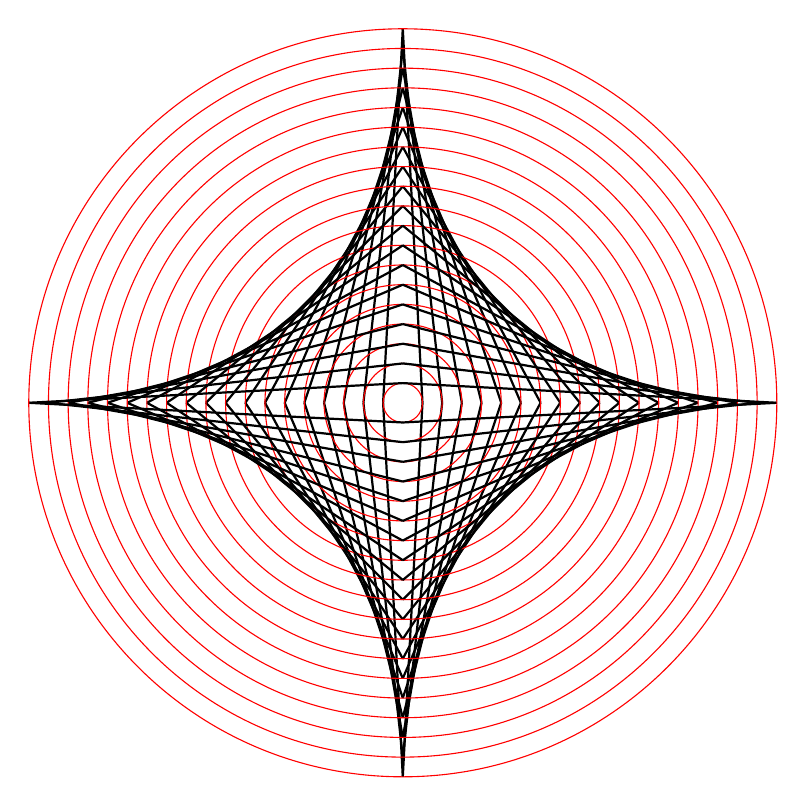
\begin{tikzpicture}[scale=0.5]
	\foreach \x in {0.5 , 1 , 1.5 , 2 ,..., 9.5} {
			\draw[thick] (-\x,0) -- (0, 10 -\x);
			\draw[thick] (\x,0) -- (0, 10 -\x);
			\draw[thick] (-\x,0) -- (0, \x-10);
			\draw[thick] (\x,0) -- (0, \x-10);
			\draw[red] (0,0) circle (\x);
		}
\end{tikzpicture}

% %! TEX root = ../../../1techno.tex
\chapter{Proportion et évolution pourcentage}

\section{Proportion et pourcentage}

\subsection{Proportion}

\begin{defn}[Proportion]
	Soit une \textbf{sous-population} de taille $n$ incluse dans une \textbf{population totale} (de référence) de taille $N$.

	La \textbf{proportion} de la sous-population est :
	\[
		p = \dfrac{n}{N}
	\]

	Elle peut s'exprimer en \textbf{pourcentage} en multipliant par $100$.

	\begin{center}
		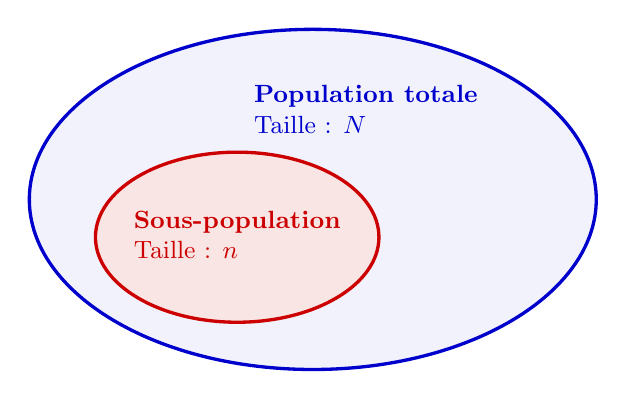
\begin{tikzpicture}[scale=1.2, every node/.style={font=\small}]
			\colorlet{popColor}{blue!80!black}
			\colorlet{subColor}{red!80!black}
			\draw[popColor, very thick, fill=popColor!5] (0,0) ellipse (3cm and 1.8cm);
			\node[anchor=south west, popColor] at (-0.9,0.5) {
				\begin{tabular}{l}
					\textbf{Population totale} \\
					{Taille :} $N$
				\end{tabular}
			};
			\draw[subColor, very thick, fill=subColor!10] (-0.8,-0.4) ellipse (1.5cm and 0.9cm);
			\node[anchor=center, subColor] at (-0.8,-0.4) {
				\begin{tabular}{l}
					\textbf{Sous-population} \\
					{Taille :} $n$
				\end{tabular}
			};
		\end{tikzpicture}
	\end{center}
\end{defn}

\begin{ex}
	Sur $480$ élèves inscrits en classe de 1\up{re}, $108$ d'entre eux sont en STMG.

	La proportion d'élèves de STMG parmi tous les élèves de 1\up{re} est :
	\[
		p = \dfrac{108}{480} = \dfrac{9}{40} = 0,225 = 22,5\,\%
	\]
\end{ex}

\begin{prop}[Pourcentage d'un nombre]
	La proportion d'une sous-population (d'effectif $n$) parmi une population totale (d'effectif $N$) est :
	\[
		{p = \dfrac{n}{N}} \quad \text{et en pourcentage :} \quad {p_{\%}=\dfrac{n}{N}\times 100}
	\]
\end{prop}

\begin{rem}
	Pour calculer un effectif $n$ ou un effectif total $N$ à l'aide d'une proportion $p$, on utilise les relations :
	\[
		{n = p \times N} \quad \text{ou} \quad {N = \dfrac{n}{p}}
	\]
\end{rem}

\begin{ex}
	Parmi les $480$ élèves de 1\up{re}, $15\,\%$ ont choisi l'option anglais renforcé. Le nombre d'élèves concernés est :
	\[
		15\,\% \times 480 = \dfrac{15}{100} \times 480 = 72 \text{ élèves}
	\]
\end{ex}

\begin{methode}[Associer effectif, proportion et pourcentage]
	Une société de $75$ employés compte $12\,\%$ de cadres et le reste d'ouvriers. $35$ employés de cette société sont des femmes et $5$ d'entre elles sont cadres.
	\begin{enumerate}
		\item Calculer l'effectif des cadres.
		\item Calculer la proportion de femmes dans cette société.
		\item Calculer la proportion, en $\%$, de cadres parmi les femmes. Les femmes cadres sont-elles sous ou surreprésentées dans cette société ?
	\end{enumerate}

	\begin{correction}
		\begin{enumerate}
			\item $12\,\%$ de $75$ = $\dfrac{12}{100} \times 75 = 9$. Cette société compte $9$ cadres.
			\item La proportion de femmes est :
			      \[
				      p_{1} = \dfrac{35}{75} = \dfrac{7}{15} \approx 0,47 = 47\,\%
			      \]

			\item La population de référence est maintenant « les femmes ». La proportion de cadres parmi les femmes est :
			      \[
				      p_{2} = \dfrac{5}{35} = \dfrac{1}{7} \approx 0,14 = 14\,\%
			      \]

			      Comme $14\,\% > 12\,\%$, les femmes cadres sont surreprésentées dans cette société.
		\end{enumerate}
	\end{correction}
\end{methode}

\subsection{Pourcentage de pourcentage}

\begin{prop}[Pourcentage de pourcentage]
	Soient $3$ ensembles $A$, $B$ et $C$ tels que $A \subset B$ et $B \subset C$.

	Si $p_{1}$ est la proportion de $A$ dans $B$ et $p_{2}$ est la proportion de $B$ dans $C$, alors la proportion de $A$ dans $C$ est :
	\[
		{p_3 = p_{1} \times p_{2}}
	\]

	\begin{center}
		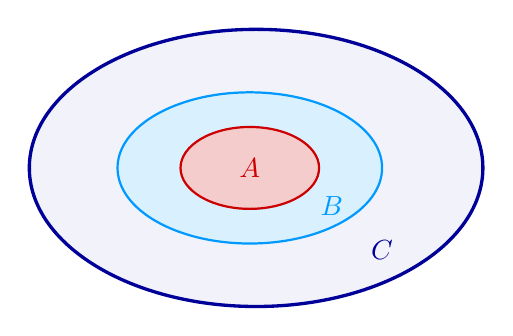
\begin{tikzpicture}[scale=0.8, every node/.style={font=\small}]
			\colorlet{cColor}{blue!60!black}
			\colorlet{bColor}{blue!40!cyan}
			\colorlet{aColor}{red!80!black}
			\draw[cColor, very thick, fill=cColor!5] (0, 0) ellipse (3.6cm and 2.2cm);
			\node[cColor, font=\bfseries] at (2.0, -1.3) {$C$};
			\draw[bColor, thick, fill=bColor!15] (-0.1, 0) ellipse (2.1cm and 1.2cm);
			\node[bColor, font=\bfseries] at (1.2, -0.6) {$B$};
			\draw[aColor, thick, fill=aColor!20] (-0.1, 0) ellipse (1.1cm and 0.65cm);
			\node[aColor, font=\bfseries] at (-0.1, 0) {$A$};
		\end{tikzpicture}
	\end{center}
\end{prop}

\begin{rem}
	Pour calculer un pourcentage de pourcentage, on multiplie les pourcentages entre eux.
\end{rem}

\begin{ex}
	Dans un bus, il y a $40\,\%$ de scolaires. Parmi les scolaires, $60\,\%$ sont des filles.

	La proportion de filles scolaires dans le bus est :
	\[
		60\,\%\text{ de } 40\,\% = 0,6 \times 0,4 = 0,24 = 24\,\%
	\]
\end{ex}

\section{Évolution exprimée en pourcentage}

\subsection{Taux d'évolution}

\begin{defn}[Taux d'évolution]
	On considère une valeur initiale $V_i$ qui subit une évolution pour arriver à une valeur finale $V_f$.

	Le \textbf{taux d'évolution} $t$ est donné par :
	\[
		{t = \dfrac{V_f - V_i}{V_i}}
	\]

	En pourcentage, le taux d'évolution est $t_{\%} = \dfrac{V_f - V_i}{V_i} \times 100$.

	\begin{center}
		\begin{tikzpicture}[>=Stealth, node distance=2.2cm, thick]
			\tikzstyle{valeur} = [font=\large\bfseries]
			\tikzstyle{taux} = [draw=blue!70, fill=blue!10, rounded corners=6pt, inner sep=6pt, font=\large\bfseries, text=blue!90!black]
			\node[valeur] (Vi) {$V_i$};
			\node[taux, right of=Vi] (T) {Taux $t$};
			\node[valeur, right of=T] (Vf) {$V_f$};
			\draw[->, line width=1.2pt, blue!70] (Vi) -- (T);
			\draw[->, line width=1.2pt, blue!70] (T) -- (Vf);
		\end{tikzpicture}
	\end{center}
\end{defn}

\begin{rem}
	\nline
	\begin{itemize}
		\item Si $t > 0$, l'évolution est une augmentation.
		\item Si $t < 0$, l'évolution est une diminution.
	\end{itemize}
\end{rem}

\begin{ex}
	La population d'un village est passée de $\np{8500}$ à $\np{10400}$. Le taux d'évolution est :
	\[
		t = \dfrac{10400 - 8500}{8500} \approx 0,224 = +22,4\,\%
	\]
\end{ex}

\subsection{Coefficient multiplicateur et taux d'évolution}

\begin{prop}[Coefficient multiplicateur]
	Faire évoluer une valeur de $\pm t\,\%$ revient à la multiplier par le nombre $\left(1 + \dfrac{t}{100}\right)$, appelé \textbf{coefficient multiplicateur} ($CM$) :
	\[
		{CM = 1 + \dfrac{t}{100}} \quad \text{et} \quad {t = (CM - 1) \times 100}
	\]

	\begin{center}
		\begin{tikzpicture}[>=Stealth, node distance=2.5cm, thick]
			\tikzstyle{valeur} = [font=\large\bfseries]
			\tikzstyle{taux} = [draw=blue!70, fill=blue!10, rounded corners=6pt, inner sep=6pt, font=\large\bfseries, text=blue!90!black]
			\node[valeur] (Vi) {$V_i$};
			\node[taux, right of=Vi] (T) {Taux $t$};
			\node[valeur, right of=T] (Vf) {$V_f$};
			\draw[->, line width=1.2pt, blue!70] (Vi) -- (T);
			\draw[->, line width=1.2pt, blue!70] (T) -- (Vf);
			\draw[->, line width=1.2pt, blue!80!black, bend right=35] (Vi) to node[below, yshift=-2pt, font=\large\bfseries] {$\times \text{CM}$} (Vf);
		\end{tikzpicture}
	\end{center}
\end{prop}

\begin{ex}
	Le prix d'un survêtement est de $49\eur{}$. Il augmente de $8\,\%$. Son nouveau prix est :
	\[
		CM = 1 + \dfrac{8}{100} = 1,08 \quad \text{et} \quad 49 \times 1,08 = 52,92\eur{}
	\]
\end{ex}

\begin{ex}
	Le prix d'un polo est de $21\eur{}$. Il diminue de $12\,\%$. Son nouveau prix est :
	\[
		CM = 1 + \dfrac{-12}{100} = 0,88 \quad \text{et} \quad 21 \times 0,88 = 18,48\eur{}
	\]
\end{ex}

\section{Évolutions successives et taux global}

\subsection{Taux d'évolution global}

\begin{prop}[Évolutions successives]
	Si une grandeur subit des évolutions successives de coefficients multiplicateurs $CM_1$, $ CM_2$, $ CM_3$, $\ldots$ alors le \textbf{coefficient multiplicateur global} $CM_g$ est le produit de ces coefficients :
	\[
		{CM_g = CM_1 \times CM_2 \times CM_3 \times \ldots}
	\]

	\begin{center}
		\begin{tikzpicture}[>=Stealth, thick, scale=0.85, every node/.style={transform shape}]
			\tikzstyle{valeur} = [font=\large\bfseries]
			\tikzstyle{taux} = [draw=blue!70, fill=blue!10, rounded corners=5pt, inner sep=5pt, font=\small\bfseries, text=blue!90!black]
			\node[valeur] (V0) {$V_0$};
			\node[taux, right of=V0, xshift=0.8cm] (T1) {$CM_1$};
			\node[valeur, right of=T1, xshift=0.8cm] (V1) {$V_1$};
			\node[taux, right of=V1, xshift=0.8cm] (T2) {$CM_2$};
			\node[valeur, right of=T2, xshift=0.8cm] (V2) {$V_2$};
			\draw[->, line width=1pt, blue!70] (V0) -- (T1);
			\draw[->, line width=1pt, blue!70] (T1) -- (V1);
			\draw[->, line width=1pt, blue!70] (V1) -- (T2);
			\draw[->, line width=1pt, blue!70] (T2) -- (V2);
			\draw[->, line width=1.2pt, red!70!black, bend left=30] (V0) to node[above, yshift=2pt] {$CM_g = CM_1 \times CM_2$} (V2);
		\end{tikzpicture}
	\end{center}
\end{prop}

\begin{ex}
	Une valeur subit une baisse de $20\,\%$ puis une hausse de $30\,\%$.
	\[
		CM_1 = 0,8 \quad \text{et} \quad CM_2 = 1,3
	\]

	Le coefficient multiplicateur global est :
	\[
		CM_g = 0,8 \times 1,3 = 1,04
	\]

	Le taux global d'évolution est $t_g = (1,04 - 1) \times 100 = +4\,\%$ (soit une augmentation de $4\,\%$).
\end{ex}

\subsection{Taux d'évolution réciproque}

\begin{defn}[Évolution réciproque]
	On considère le taux $t$ d'évolution d'une valeur $V_0$ à une valeur $V_1$. L'\textbf{évolution réciproque} est le taux $t'$ permettant de revenir de $V_1$ à $V_0$.
\end{defn}

\begin{prop}[Coefficient multiplicateur réciproque]
	L'évolution réciproque possède un coefficient multiplicateur $CM_R$ inverse du coefficient multiplicateur direct $CM$ :
	\[
		{CM_R = \dfrac{1}{CM}}
	\]

	\begin{center}
		\begin{tikzpicture}[>=Stealth, node distance=2.2cm, thick]
			\tikzstyle{valeur} = [font=\large\bfseries]
			\tikzstyle{taux} = [draw=blue!70, fill=blue!20!white, rounded corners=3pt, inner sep=6pt, font=\large\bfseries, text=black]
			\node[valeur] (V0) {$V_0$};
			\node[taux, right of=V0] (T) {$CM$};
			\node[valeur, right of=T] (V1) {$V_1$};
			\draw[->, line width=1.2pt, blue!70!cyan] (V0) -- (T);
			\draw[->, line width=1.2pt, blue!70!cyan] (T) -- (V1);
			\draw[->, line width=1.3pt, blue!60!black, bend right=35] (V0) to node[below, yshift=-4pt] {$\times CM$} (V1);
			\draw[->, line width=1.3pt, blue!60!black, bend right=35] (V1) to node[above, yshift=4pt] {$\times CM_R = \dfrac{1}{CM}$} (V0);
		\end{tikzpicture}
	\end{center}
\end{prop}

\begin{ex}
	Le coefficient multiplicateur réciproque d'une baisse de $20\,\%$ ($CM = 0,8$) est :
	\[
		CM_R = \dfrac{1}{0,8} = 1,25
	\]

	Cela correspond à une augmentation de $t_R = (1,25 - 1) \times 100 = +25\,\%$. Pour compenser une baisse de $20\,\%$, il faut donc une augmentation de $25\,\%$.
\end{ex}

\section{Indices base 100}

\subsection{Définition et calcul d'un indice}

\begin{defn}[Indice base 100]
	L'\textbf{indice} d'une valeur $y_2$ par rapport à une valeur de référence $y_1$ (choisie comme base 100) est la valeur qu'aurait $y_2$ si $y_1$ valait $100$.

	Le tableau de correspondance est un tableau de proportionnalité :
	\def\arraystretch{1.5}
	\begin{center}
		\begin{tabular}{c|c}
			Valeurs           & Indices \\ \hline
			$y_1$ (référence) & $100$   \\ \hline
			$y_2$             & $I$     \\
		\end{tabular}
	\end{center}

	L'indice $I$ se calcule par la formule :
	\[
		{I = 100 \times \dfrac{y_2}{y_1}}
	\]
\end{defn}

\begin{prop}[Lien entre indice, taux et coefficient multiplicateur]
	Soit $I$ l'indice d'une valeur associé à un taux d'évolution $t$ et un coefficient multiplicateur $CM$ :
	\[
		I = 100 \times CM = 100 \times (1 + t) \quad \text{et} \quad t = \dfrac{I}{100} - 1
	\]
\end{prop}

\begin{ex}
	Le prix d'un article passe de $350\eur{}$ à $364\eur{}$.

	Le taux d'évolution est :
	\[
		t = \dfrac{364 - 350}{350} = \dfrac{14}{350} = 0,04 = +4\,\%
	\]

	L'indice de ce prix final base 100 en $350\eur{}$ est :
	\[
		I = 100 \times \dfrac{364}{350} = 104
	\]

	Cela signifie que le prix a augmenté de $4\,\%$.
\end{ex}

\begin{methode}[Calculer et interpréter des indices]
	Le tableau ci-dessous indique l'évolution du nombre de visiteurs d'un site web entre 2017 et 2019 :
	\begin{center}
		\def\arraystretch{1.5}
		\begin{tabular}{|l|c|c|c|}
			\hline
			Année                   & 2017        & 2018        & 2019        \\ \hline
			Nombre de visites       & $\np{4376}$ & $\np{5149}$ & $\np{4813}$ \\ \hline
			Indice base 100 en 2017 & $100$       & $\dots$     & $\dots$     \\ \hline
		\end{tabular}
	\end{center}

	Calculer les indices pour les années 2018 et 2019 en prenant 2017 comme base 100.

	\begin{correction}
		\nline

		\begin{itemize}
			\item Pour 2018 :
			      \[
				      I_{2018} = 100 \times \dfrac{5149}{4376} \approx 117,7
			      \]
			\item Pour 2019 :
			      \[
				      I_{2019} = 100 \times \dfrac{4813}{4376} \approx 110,0
			      \]
		\end{itemize}

		\textbf{Interprétation :}
		\begin{itemize}
			\item L'indice $117,7$ en 2018 indique une hausse de $17,7\,\%$ du nombre de visites par rapport à 2017.
			\item L'indice $110$ en 2019 traduit une hausse globale de $10\,\%$ par rapport à l'année de référence 2017.
		\end{itemize}
	\end{correction}
\end{methode}

% \chapter{Fonctions affines}

\section{Introduction et exemple concret}

\begin{ex}[Situation des compagnies de bus]
	Pour un voyage scolaire, une classe de Première STMG compare les tarifs de deux compagnies de transport :
	\begin{itemize}
		\item \textbf{Compagnie A :} applique un forfait fixe de $15\eur{}$ auquel s'ajoute $2\eur{}$ par kilomètre parcouru.
		\item \textbf{Compagnie B :} ne facture pas de forfait fixe, mais facture $3,50\eur{}$ par kilomètre parcouru.
	\end{itemize}

	Si on note $x$ le nombre de kilomètres parcourus :
	\begin{itemize}
		\item Le prix payé avec la compagnie A est : $f(x) = 2x + 15$.
		\item Le prix payé avec la compagnie B est : $g(x) = 3,50x$.
	\end{itemize}

	Les fonctions $f$ et $g$ ainsi définies sont des \textbf{fonctions affines}.
\end{ex}

\section{Définitions et vocabulaire}

\subsection{Fonction affine}

\begin{defn}[Fonction affine]
	Soit $m$ et $p$ deux nombres réels donnés.

	Une \textbf{fonction affine} $f$ est une fonction définie sur $\R$ par l'expression :
	\[
		f(x) = mx + p
	\]

	\begin{itemize}
		\item Le nombre $m$ est appelé le \textbf{coefficient directeur}.
		\item Le nombre $p$ est appelé l'\textbf{ordonnée à l'origine}.
	\end{itemize}
\end{defn}

\begin{rem}[Cas particuliers]
	\nline
	\begin{itemize}
		\item Si $p = 0$, alors $f(x) = mx$ : on dit que $f$ est une \textbf{fonction linéaire} (situation de proportionnalité).
		\item Si $m = 0$, alors $f(x) = p$ : on dit que $f$ est une \textbf{fonction constante}.
	\end{itemize}
\end{rem}

\begin{ex}
	\nline
	\begin{itemize}
		\item $f(x) = 3x - 5$ est une fonction affine avec $m = 3$ et $p = -5$.
		\item $g(x) = -2x + 7$ est une fonction affine avec $m = -2$ et $p = 7$.
		\item $h(x) = 4x$ est une fonction affine (et linéaire) avec $m = 4$ et $p = 0$.
		\item $k(x) = 6$ est une fonction affine (et constante) avec $m = 0$ et $p = 6$.
	\end{itemize}
\end{ex}

\subsection{Calcul d'une image et d'un antécédent}

\begin{methode}[Calculer une image ou un antécédent]
	Soit la fonction affine $f(x) = 2x + 15$ (tarifs de la compagnie A).
	\begin{enumerate}
		\item Calculer le prix pour un trajet de $40\text{ km}$ (image de $40$).
		\item Déterminer le nombre de kilomètres parcourus pour un montant de $55\eur{}$ (antécédent de $55$).
	\end{enumerate}

	\begin{correction}
		\nline
		\begin{enumerate}
			\item On calcule $f(40)$ :
			      \[
				      f(40) = 2 \times 40 + 15 = 80 + 15 = 95
			      \]
			      Le prix pour $40\text{ km}$ est de $95\eur{}$.

			\item On cherche $x$ tel que $f(x) = 55$ :
			      \[
				      2x + 15 = 55 \eqv 2x = 40 \eqv x = 20
			      \]
			      Pour un montant de $55\eur{}$, la distance parcourue est de $20\text{ km}$.
		\end{enumerate}
	\end{correction}
\end{methode}

\section{Représentation graphique}

\begin{prop}[Représentation graphique d'une fonction affine]
	Dans un repère du plan, la représentation graphique d'une fonction affine $f(x) = mx + p$ est une \textbf{droite}.
	\begin{itemize}
		\item $p$ est l'ordonnée du point d'intersection de la droite avec l'axe vertical $(0\,;\,p)$.
		\item Le coefficient directeur $m$ caractérise la pente de la droite.
	\end{itemize}
\end{prop}

% TODO illustration à revoir
\begin{center}
	\begin{tikzpicture}[>=Stealth]
		\draw[->] (-1,0) -- (5,0) node[above] {$x$};
		\draw[->] (0,-1) -- (0,4) node[right] {$y$};
		\draw[ultra thick, blue, domain=-1:5] plot ( \x , 0.5*\x+1 );
		% \draw[thick, blue] (-0.5,0.5) -- (4.5,4.5) node[right] {$y = mx + p$};
		\fill (0,1) circle (3pt) node[above left] {$p$};
		\draw[dashed] (1,1.5) -- (3,1.5) -- (3,2.5);
		\node at (2,1.2) {$1$};
		\node at (3.4,2) {$m$};
	\end{tikzpicture}
\end{center}
\begin{methode}[Tracer la droite représentant une fonction affine]
	Pour tracer la droite représentant la fonction $f(x) = 2x + 15$ sur l'intervalle $[0\,;\,30]$ :
	\begin{enumerate}
		\item On calcule les coordonnées de deux points (par exemple pour $x = 0$ et $x = 20$) :
		      \begin{itemize}
			      \item Si $x = 0$, $f(0) = 2(0) + 15 = 15$ (Point $A(0\,;\,15)$).
			      \item Si $x = 20$, $f(20) = 2(20) + 15 = 55$ (Point $B(20\,;\,55)$).
		      \end{itemize}
		\item On place ces deux points dans le repère et l'on trace la droite passant par $A$ et $B$.
	\end{enumerate}
\end{methode}

\section{Sens de variation}

\begin{prop}[Sens de variation d'une fonction affine]
	Soit $f(x) = mx + p$ une fonction affine sur $\R$. Le sens de variation de $f$ dépend du signe de son coefficient directeur $m$ :
	\begin{itemize}
		\item Si $m > 0$, la fonction $f$ est \textbf{croissante} sur $\R$.
		\item Si $m < 0$, la fonction $f$ est \textbf{décroissante} sur $\R$.
		\item Si $m = 0$, la fonction $f$ est \textbf{constante} sur $\R$.
	\end{itemize}
\end{prop}

\begin{ex}
	\nline
	\begin{itemize}
		\item Pour la fonction $f(x) = 2x + 15$ (compagnie A), on a $m = 2 > 0$ : la fonction est \textbf{croissante}. Plus on roule, plus le prix augmente.
		\item Pour la fonction $g(x) = -1,5x + 50$, on a $m = -1,5 < 0$ : la fonction est \textbf{décroissante}.
	\end{itemize}
\end{ex}

\begin{prop}[Tableau de variation]
	Voici l'allure générale du tableau de variation d'une fonction affine selon le signe de $m$ :

	\begin{center}
		\begin{tabular}{cc}
			\textbf{Si $m > 0$ (Croissante)} & \textbf{Si $m < 0$ (Décroissante)} \\
			\begin{tikzpicture}
				\tkzTabInit[lgt=1,espcl=2.5]{$x$ / 1, $f$ / 2}{$-\infty$, $+\infty$}
				\tkzTabVar{-/ , +/}
			\end{tikzpicture}
			                                 &
			\begin{tikzpicture}
				\tkzTabInit[lgt=1,espcl=2.5]{$x$ / 1, $f$ / 2}{$-\infty$, $+\infty$}
				\tkzTabVar{+/ , -/}
			\end{tikzpicture}
		\end{tabular}
	\end{center}
\end{prop}

\section{Étude du signe}

\begin{prop}[Signe d'une expression affine]
	Soit $f(x) = mx + p$ avec $m \neq 0$.
	L'expression s'annule pour la valeur (appelée racine) :
	\[
		x = -\dfrac{p}{m}
	\]
	Le signe de $mx + p$ est donné par la règle suivante : \textbf{le signe de $m$ après la racine, et le signe contraires de $m$ avant la racine}.
\end{prop}

\begin{methode}[Établir le tableau de signes]
	Pour étudier le signe de $f(x) = 2x - 6$ :
	\begin{enumerate}
		\item On résout l'équation $2x - 6 = 0 \eqv 2x = 6 \eqv x = 3$.
		\item Le coefficient directeur est $m = 2 > 0$.
	\end{enumerate}
	Le tableau de signes est donc :
	\begin{center}
		\begin{tikzpicture}
			\tkzTabInit[lgt=2,espcl=3]{$x$ / 1, $2x - 6$ / 1}{$-\infty$, $3$, $+\infty$}
			\tkzTabLine{,-,0,+,}
		\end{tikzpicture}
	\end{center}
\end{methode}

\section{Résolution d'équations et d'inéquations}

\subsection{Résolution d'une équation $f(x) = g(x)$}

\begin{methode}[Résoudre $f(x) = g(x)$]
	Revenons à nos deux compagnies de bus avec :

	\begin{itemize}
		\item $f(x) = 2x + 15$ (Compagnie A)
		\item $g(x) = 3,50x$ (Compagnie B)
	\end{itemize}

	À partir de combien de kilomètres les deux compagnies coûtent-elles exactement le même prix ?

	\begin{correction}
		On résout l'équation $f(x) = g(x)$ :
		\[
			2x + 15 = 3,50x
		\]
		\[
			15 = 3,50x - 2x
		\]
		\[
			15 = 1,50x
		\]
		\[
			x = \dfrac{15}{1,50} = 10
		\]
		Pour un trajet de $10\text{ km}$, les deux compagnies coûtent le même prix ($35\eur{}$).
	\end{correction}
\end{methode}

\subsection{Résolution d'une inéquation $f(x) < g(x)$}

\begin{methode}[Résoudre une inéquation entre fonctions affines]
	En reprenant les compagnies A et B, à partir de quelle distance la compagnie A devient-elle plus avantageuse que la compagnie B ?

	\begin{correction}
		On cherche à résoudre l'inéquation $f(x) < g(x)$ :
		\[
			2x + 15 < 3,50x
		\]
		\[
			15 < 3,50x - 2x
		\]
		\[
			15 < 1,50x
		\]
		\[
			x > \dfrac{15}{1,50} \eqv x > 10
		\]
		La compagnie A est plus avantageuse pour un nombre de kilomètres \textbf{strictement supérieur à $10\text{ km}$}.
	\end{correction}
\end{methode}

\end{document}
